%%
%% This is file `mcmthesis-demo.tex',
%% generated with the docstrip utility.
%%
%% The original source files were:
%%
%% mcmthesis.dtx  (with options: `demo')
%%
%% -----------------------------------
%%
%% This is a generated file.
%%
%% Copyright (C)
%%     2010 -- 2015 by Zhaoli
%%     2014 -- 2016 by Liam 
%%     2017 -- 2019 by Xuehan
%%
%% This work may be distributed and/or modified under the
%% conditions of the LaTeX Project Public License, either version 1.3
%% of this license or (at your option) any later version.
%%
%% This work has the LPPL maintenance status `maintained'.
%%
%% The Current Maintainer of this work is Xuehan.
%%
\documentclass{mcmthesis}
\bibliographystyle{IEEEtran}
\mcmsetup{CTeX = false,   % 使用 CTeX 套装时,设置为 true
        tcn = 2002134, problem = D,
        sheet = true, titleinsheet = true, keywordsinsheet = true,
        titlepage = true}
\usepackage{palatino}
\usepackage{mwe}
\usepackage{graphicx}
\usepackage{subcaption}
\usepackage{float}
\usepackage{multirow}
\usepackage{indentfirst}
\usepackage{gensymb}
\usepackage[ruled,lined,commentsnumbered]{algorithm2e}
\usepackage{geometry}


\begin{document}
\linespread{0.6} %%行间距
\setlength{\parskip}{0.5\baselineskip} %%段间距
\title{ti}

\date{\today}
	\begin{abstract}

	
		\begin{keywords}
		
		\end{keywords}
	\end{abstract}

\maketitle

\tableofcontents

\newpage

\section{Introduction}
\subsection{Problem Background}
	Football is one of the most well-known sports activities in the world.  The standard system of an 11-man football game is one goalkeeper and 10 players from each of the two teams. There are a total of 22 players who fight, defend and attack on the rectangular grass court.  The game scores by shooting the ball into the opponent's goal. When the game is over, the team with the most points wins.

	\begin{figure}[h]
		\centering
		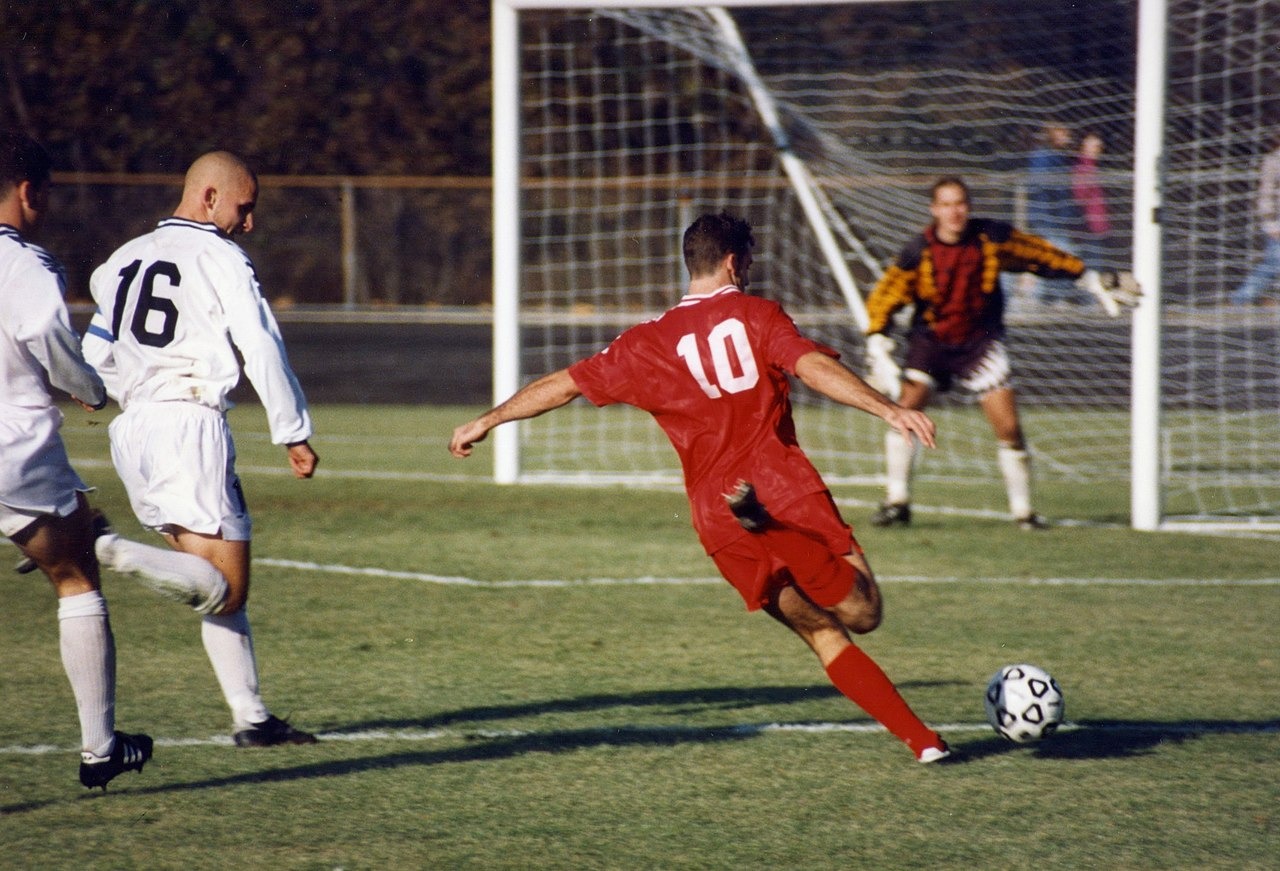
\includegraphics[width=0.75\textwidth]{figures/football.jpg}
		\caption{A Football Game~\cite{Wiki_Football}}
		\label{fig:football}
	\end{figure}

	As we all know, football is a sport that requires intense teamwork.  For it can show the importance of teamwork spirit more than superb personal ability.  Passing, as an offensive means that requires the cooperation of various players to play the biggest role, is just an important manifestation of the team spirit of football.  Therefore, to study the important role of teamwork in football, you can start by studying the passing network in football.

	Our goal is to build a network model to simulate the Huskies' passing network and study it.  Meanwhile, it is necessary to extract some representative parameters from the constructed network model.  Through the study of such parameters, we can accurately understand the team collaboration ability and structural characteristics of this team.
\subsection{Our Work}
	In this paper, we successfully built the Huskies' passing network model.  On the basis of this network model, we obtained some important parameters. In this way, we analyzed the team collaboration ability of the Huskies players, and offered some suggestion for its future structural strategy.

	In Section 2, we state some basic assumptions.  Section 3 contains the nomenclature used in the statement of our model.  Section 4 provides sufficient details about our network model.  Section 5 carries on the simulation experiment and analysis to our proposed model.  Section 6 provides some advice on its structural strategies for the Huskies.  Finally, we further analyze the sensitivity, advantages and disadvantages of our model in Section 7, and we obtain some conclusions on how to improve the teamwork spirit of general teams in Section 8.
\section{Assumptions}
	Our model is based on these following basic assumptions:
	\begin{enumerate}
		\item The average position of a player over a period of time is equivalent to the average of the position of the player in all events that occurred during that period.
		\item We consider a dyadic configuration tight if players in this dyadic configuration continuously pass each other far more often than they pass other players.  The same is true for triadic configurations.
	\end{enumerate}
\section{Nomenclature}
	Symbols that our model mainly uses are listed in Table \ref{tab:Nomen}.  Other symbols that are used only once will be described in the following chapters.
	\begin{table}
    	\centering
    	\caption{Nomenclature}
		\label{tab:Nomen}
		\begin{tabular}{c c}
			\hline	
				Symbol & Definition\\
			\hline
				$\textbf{A}$ & Football passing matrix\\
				$\textbf{B}$ & Adjacency matrix\\
				$G$ & Undirected graph representing the football passing network\\
				$p_{i}$ & The \emph{i}th player in Huskies\\
				$p_{ij}$ & Number of passes from player $i$ to player $j$\\
				$\langle$$X$$\rangle$ & The x-coordinate of the network centroid\\
				$\langle$$Y$$\rangle$ & The y-coordinate of the network centroid\\
				$D$ & The dispersion of the position of the players around the network centroid\\
			\hline
   	 	\end{tabular}
	\end{table}

\section{The Basic Model}
	In this section we will discuss our network model in detail.  First of all, we will begin with the establishment of our network model.  Then we will use our model to identify some patterns of the network.  Finally, we will also investigate the indicators of teamwork. 
\subsection{Build of the Network}
	First of all, we define Huskies' football passing matrix $\textbf{A}$.  When the number of players who have played is $n$, $\textbf{A}$ is a square matrix of $n \times n$, which is defined as:
	\begin{equation}\label{eq:Mat_A}
		a_{ij} =
		\begin{cases}
			p_{ij}& \text{$i \neq j$}\\
			0& \text{$i = j$}
		\end{cases}
	\end{equation}
	In this way, we obtain an asymmetric square matrix of order $n$.  Next, on this basis, we try to build an undirected graph model to describe the team's passing network.  But as we have mentioned before, the adjacency matrix of an undirected graph is a symmetric matrix, while the football passing matrix $\textbf{A}$ we constructed is asymmetric.  Therefore, we need to construct a symmetric adjacency matrix $\textbf{B}$ using this asymmetric passing matrix $\textbf{A}$.  To achieve this, we define $\textbf{B}$ as the sum of $\textbf{A}$ and the transposed matrix of $\textbf{A}$, that is to say, for each element $b_{ij}$ in B, the following formula is satisfied:
	\begin{equation}
		\label{eq:Mat_B}
		b_{ij} = a_{ij} + a_{ji}
	\end{equation}
	Now we can easily find that $\textbf{B}$ is equal to its transpose matrix.  Hence $\textbf{B}$ is a symmetric matrix.

	After getting $\textbf{B}$, we can continue to study the undirected graph $G$.  From the previous definition of the adjacency matrix, it can be seen that the nodes in this undirected graph represent the Huskies players, and the edges represent interactions between players.  For quantitative research, we define the weight of node $i$ in the undirected graph $G$ as the sum of the number of passes and catches by player $i$, and the weight of edge $E (i, j)$ is defined as the sum of the number of passes from player $i$ to player $j$ and the number of passes from player $j$ to player $i$.
	
	In order to have an intuitive understanding of the football passing network, we can draw this undirected graph on a schematic diagram of a football field.  Among them, circles represent nodes, and straight lines connecting circles represent edges.  For a node, the larger its size and the darker its color, the greater the weight of the node.  For an edge, the thicker its thickness and the darker its color, the greater the weight of the edge.  In addition, in order to gain a clear understanding of the formation and other factors of this team, we plot the nodes on the represented player's the average position in the studied period.  In this way, we obtain a schematic diagram which can intuitively reflect the football passing network.  Figure \ref{fig:playground} is an example by us.
	
	\begin{figure}[h]
		\centering
		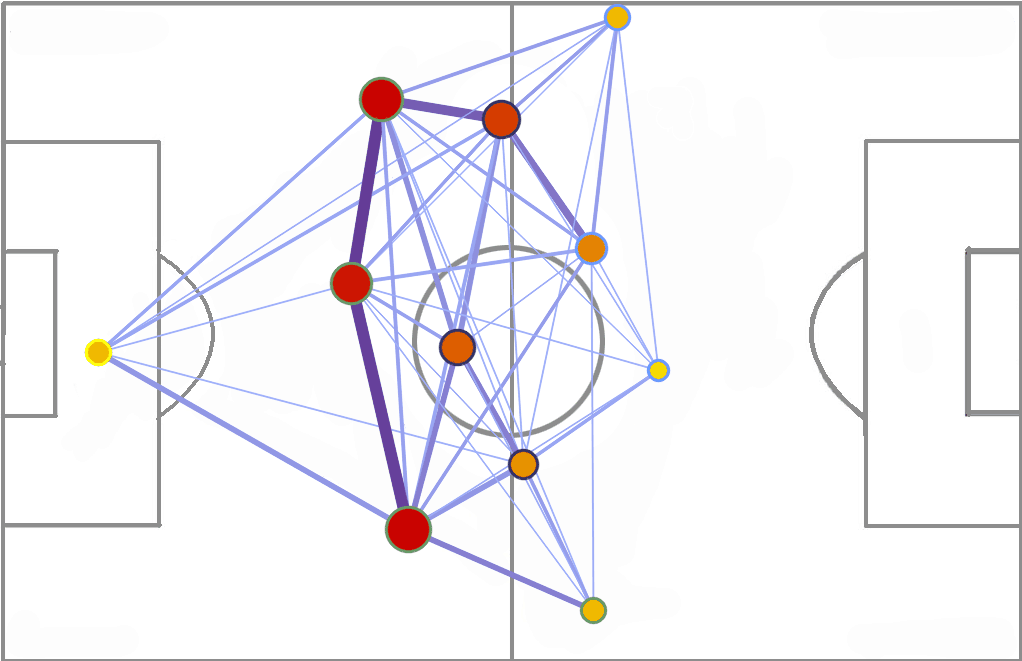
\includegraphics[width=\textwidth]{figures/playground.png}
		\caption{An Example of the Football Passing Network}
		\label{fig:playground}
	\end{figure}
\subsection{Identify Network Patterns}
	After establishing the football passing network, we will use this model to identify some special patterns of Huskies' network.  In the following chapters, we will investigate Huskies' continuous football passing chain, network centroid and advance ratio to identify its patterns on multiple scales. 
\subsubsection{Continuous Football Passing Chain}
	Just as we have stated in assumption 2, when players in a dyadic or triadic configuration continuously pass each other far more frequently than they do with other players in the team, we consider this configuration tight.  Therefore, when investigating the tightness of such configurations, we need to study the behavior of continuous passing between players.  For this reason, we construct a continuous football passing chain as a tool to study this behavior according to the football passing network.

	In football games, passing is a very continuous activity.  It can be said that before occasion like shooting, out of bounds or the football is intercepted by the opposing player occurs, the passing can build a transitive binary relationship between our players.  Therefore, we can use this characteristic to construct a continuous football passing chain, which is continuous and transitive.  The general construction method is: According to the data in passingevents, we record the process of continuous passing of football between Huskies players with a linked chain.  This chain will continue until disruptive occasions such as shooting, out of bounds or the football is intercepted by the opponent occur.  In this way, we get a chain that records the continuous passing of the Husky players.
\subsubsection{Network Centroid And Advance Ratio}
\subsection{Identify Teamwork Indicators}
\section{Implementation}
\section{Structural Strategies}
\section{Model Analysis}
\subsection{Sensitivity Analysis}
\subsection{Strengths and Weakness}
\section{Conclusion}

\bibliography{ref}
\newpage

\begin{appendices}


\end{appendices}

\end{document}
